\documentclass[urlcolor=blue,dvipsnames]{beamer}

\usepackage[utf8]{inputenc}
\usepackage{fancybox,fancyvrb}
\usepackage{environ,xspace}
\usepackage{tikz}
\hypersetup{colorlinks,linkcolor=,urlcolor=cyan}

\beamertemplatenavigationsymbolsempty
\setbeamertemplate{footline}[frame number]
\usetheme{Pittsburgh}

\newcommand\enumnum[1]{{\renewcommand{\insertenumlabel}{#1}%
      \usebeamertemplate{enumerate item} \,}}

\newcommand{\grad}{\nabla}
\newcommand{\ih}{\boldsymbol{\hat{\textbf{\i}}}}
\newcommand{\jh}{\boldsymbol{\hat{\textbf{\j}}}}
\newcommand{\vF}{\boldsymbol{\vec{\textbf{F}}}}
\newcommand{\Matlab}{\textsc{Matlab}\xspace}
\newcommand{\Octave}{\textsc{Octave}\xspace}


\title{5.3 Nonlinear models \\ (with some 4.10 material too)}

\subtitle{a lesson for MATH F302 Differential Equations}

\author{Ed Bueler, Dept.~of Mathematics and Statistics, UAF}

\date{\tiny \today}


\begin{document}
\setbeamertemplate{itemize item}{$\bullet$}
\setbeamertemplate{itemize subitem}{$\circ$}


\begin{frame}
\titlepage

\centerline{\tiny for textbook: \, D. Zill, \emph{A First Course in Differential Equations with Modeling Applications}, 11th ed.}
%\color{green!40!blue}
\end{frame}


\begin{frame}{outline}

\begin{itemize}
\item nonlinear pendulum (\S 5.3)
\item using a numerical solver in \Matlab/\Octave (see \S4.10)
\item nonlinear spring (\S 5.3)
\item non-constant gravity: from earth to high orbit (\S 5.3)
\item dependent variable missing (\S 4.10)
\end{itemize}
\end{frame}


\begin{frame}{nonlinear pendulum}

\begin{itemize}
\item X
\end{itemize}

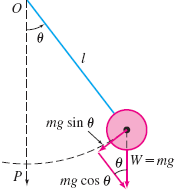
\includegraphics[width=0.4\textwidth]{figs/pendulum}
\end{frame}


\begin{frame}{X}

\begin{itemize}
\item X
\end{itemize}
\end{frame}


\begin{frame}{X}

\begin{itemize}
\item X
\end{itemize}
\end{frame}


\begin{frame}{X}

\begin{itemize}
\item X
\end{itemize}
\end{frame}


\begin{frame}{X}

\begin{itemize}
\item X
\end{itemize}
\end{frame}


\begin{frame}{X}

\begin{itemize}
\item X
\end{itemize}
\end{frame}


\begin{frame}{expectations}

\begin{itemize}
\item just watching this video is \emph{not} enough!
     \begin{itemize}
     \item see ``found online'' videos at

     \centerline{\href{https://bueler.github.io/math302/week8.html}{\tt \color{cyan} bueler.github.io/math302/week8.html}}
     \item \emph{read} section 4.10 in the textbook
         \begin{itemize}
         \item skip the ``Use of Taylor series'' material \dots we'll get to it later
         \end{itemize}
     \item \emph{read} section 5.3 in the textbook
         \begin{itemize}
         \item you can safely skip the material on ``Telephone wires'' (a boundary value problem \dots not in Math 302)
         \end{itemize}
     \item \emph{do} the WebAssign exercises for section 5.3, which include some problems from 4.10
     \end{itemize}
\end{itemize}
\end{frame}

\end{document}

